\subsubsection{重要な意思決定としてのアーキテクチャ}
アーキテクチャ設計は創造的な活動である。アーキテクトは、要求、品質特性、制約、利用可能な資源、組織の状況を踏まえ、多くの意思決定を行う。特に、品質特性のトレードオフは重要である。性能を高める選択が保守性を下げることがあり、セキュリティを高める選択が使いやすさや費用に影響することがある。

アーキテクチャは、意思決定の網として理解できる。ある決定が、次の決定の前提になる。したがって、重要な判断は、理由とともに記録する必要がある。

\begin{statementbox}{アーキテクチャ根拠}
アーキテクチャ根拠とは、なぜその決定をしたのかを説明する情報である。前提、検討した代替案、選択基準、トレードオフ、却下した案とその理由を含む。将来の保守担当者にとって、決定の理由は決定内容と同じくらい重要である。
\end{statementbox}

\keyterm{アーキテクチャ技術的負債}とは、現在のアーキテクチャ判断が将来の変更や運用に余分な費用を生む状態である。たとえば、初回リリースのためにモジュール性を十分考えずに作ると、後続リリースで機能追加のたびに大きな改修が必要になり、欠陥も増えやすい。この負債は、最初に判断した人ではなく、後から開発や保守を行う人が支払うことが多い。

\begin{figure}[htbp]
\centering
\IfFileExists{assets/generated_figures/ch02/fig-ch02-06.png}{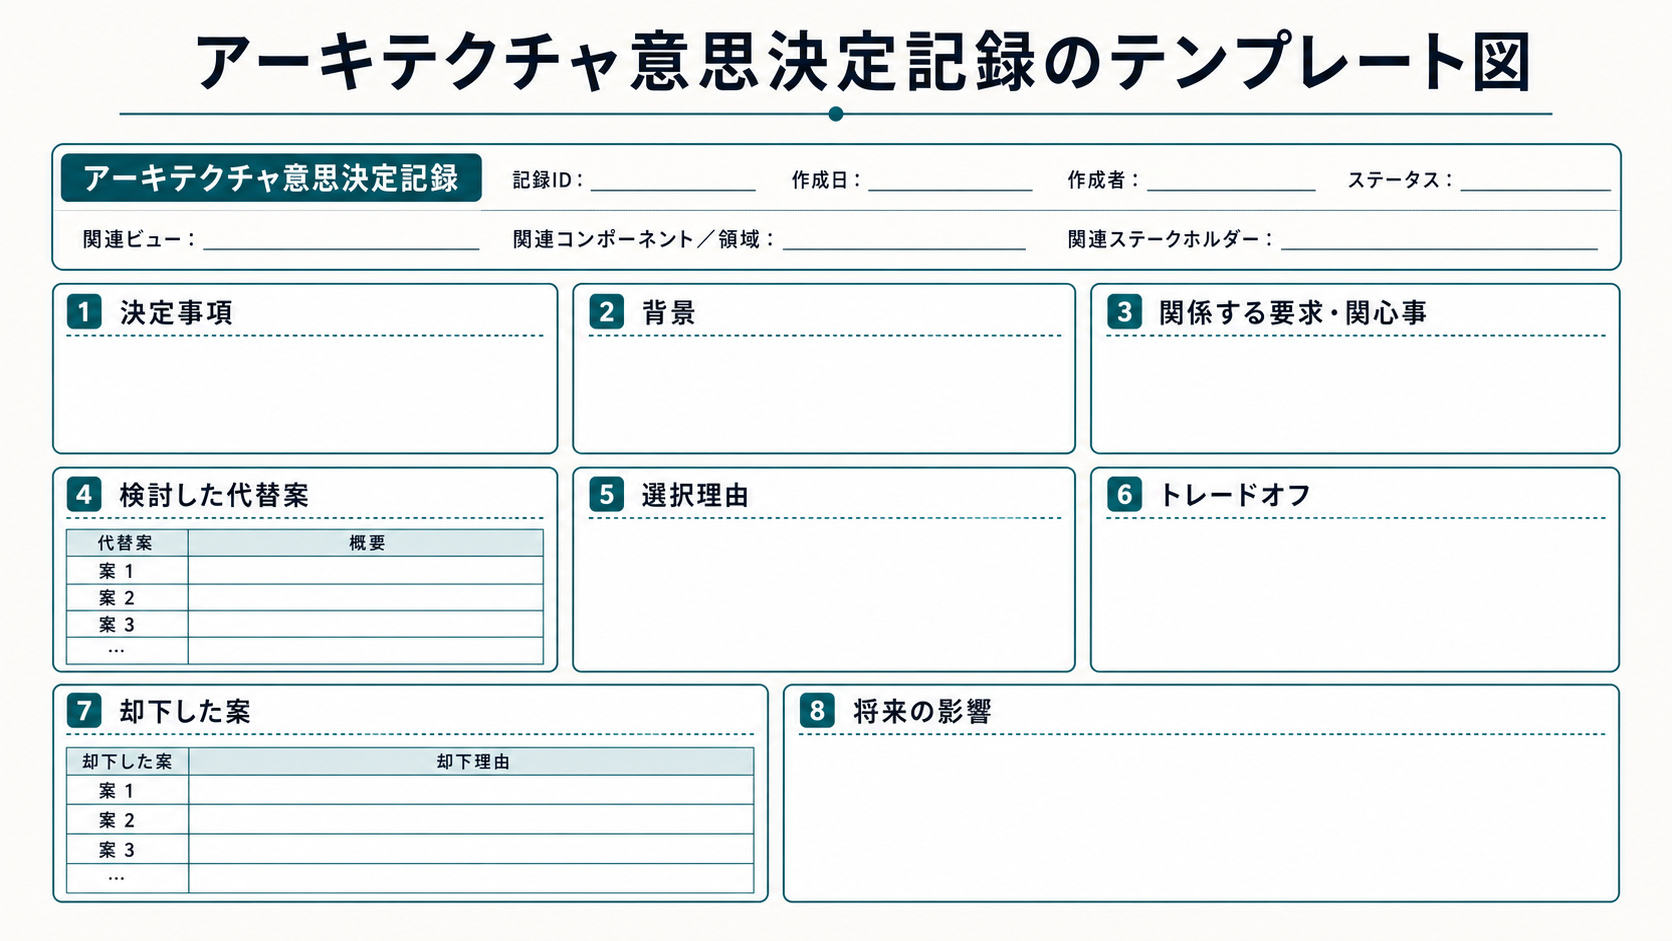
\includegraphics[width=0.96\linewidth]{assets/generated_figures/ch02/fig-ch02-06.png}}{\fbox{\parbox[c][48mm][c]{0.9\linewidth}{\centering 画像生成待ち\\アーキテクチャ意思決定記録のテンプレート図}}}
\caption{アーキテクチャ意思決定記録のテンプレート図}
\label{fig:ch02-06}
\end{figure}
